\documentclass[12pt]{report}
\usepackage[a4paper,top=15mm, bottom=25mm, left=23mm, right=23mm]{geometry}
\usepackage[english]{babel}
\usepackage[utf8]{inputenc}
\usepackage{mathptmx}
\usepackage{amssymb}
\usepackage{amsmath}
\usepackage{enumitem}
\usepackage{tikz}
\usepackage{stuki}

\renewcommand{\labelitemi}{$-$}
\renewcommand{\labelitemii}{}

\usetikzlibrary{arrows,shapes,positioning,shadows,trees}

\tikzset{
  basic/.style  = {draw, text width=3cm, drop shadow, font=\sffamily, rectangle},
  root/.style   = {basic, rounded corners=2pt, thin, align=center,
                   fill=blue!30},
  level 2/.style = {basic, rounded corners=6pt, thin,align=center, fill=blue!20,
                   text width=15em}
}

\begin{document}
\begin{tabular}{lcr}
\textbf{Lestár Norbert} & 1. beadandó / 11. feladat  & 2015. március 22. \\
\textbf{Neptun kód:} A8UZ7T \\
lestar.norbert@gmail.com \\
6. csoport \\
\end{tabular}
\paragraph{Feladat} \hspace{0pt} \\
\textit{Keressük meg melyik útlevélszámú utas fordult meg leghamarabb másodszor a határon!}
\paragraph{Specifikáció} \hspace{0pt} \\
A méréseket egy tömbben tároljuk. \newline
A = ( t : String$^{n}$, ind : $\mathbb{N}$, l : $\mathbb{L}$ ) \newline
Ef = ( t = t' ) \newline
Uf = ( Ef $\wedge$ l = ($\exists$ind = i : $\exists$ i $\in$ [1..n] : searchj(i)) ) = \\
( Ef $\wedge$ (l, ind) = $\exists$ SEARCH$_{i=2}^{n}$ searchj(i) ) \newline
 ahol searchj(i) := [1..n] $\rightarrow \mathbb{L}$ és searchj(i) = $\exists$ SEARCH$_{j=1}^{i}$ f(i) = f(j) \newline
\noindent\hfill
\begin{stukibox}[5cm]
\stm*{Lineáris keresés}
\stm[2]{m..n \rightarrow 2..n \\
\beta (i) \rightarrow searchj(i)
}
\end{stukibox}%
\hfill
\begin{stukibox}[5cm]
\stm*{Lineáris keresés}
\stm[2]{m..n \rightarrow 1..i \\
\alpha (j) \rightarrow t_{i} = t_{j}
}
\end{stukibox}%
\noindent\hfill \newline \\
\begin{stukibox}[5cm]
\stm*{l, i := hamis, 2}
\begin{WHILE}{2}{\stm*{!l $\wedge$ i $\leq$ n}}
\stm{l := searchj(i)}
\stm{i := i + 1}
\end{WHILE}
\end{stukibox}%
\hfill
\begin{stukibox}[5cm]
\stm*{l := searchj(i)}
\stm*{l, j := hamis, 1}
\begin{WHILE}{2}{\stm*{!l $\wedge$ j $\leq$ k}}
\stm{l := t[j] = t[k]}
\stm{j := j + 1}
\end{WHILE}
\end{stukibox}%
\hfill

\paragraph{Implementáció} \hspace{0pt} \\

\textit{\textbf{Adattípusok megvalósítása}} \newline
A kódoláskor a t tömböt vector$<$string$>$-ként deklaráljuk, amelynek mérete t.size() alakban érhető el. Mivel a vektor 0-tól indexelődik, ezért a tervbeli ciklusok nem a 2..n, hanem a 1..t.size(), és a 0..i intervallumot futják be. \\

\textit{\textbf{Bemenő adatok formája}} \newline
A bemenő adatokat egy szöveges állományból kell a tömbbe bemásolni. Az állományban a megadott számokat szóközökkel, tabulátor jelekkel vagy sorvége jelekkel elválasztva kell beírni. Az állomány minden sorát sorvége jel zárja le. Alapesetben a program csak természetes számokat vár, ám szöveget tartalmazó sorokat/egységeket is lekezeli. Például:\\
1500	150 \newline
250 \newline
-500 \\

\textit{\textbf{Program váz}} \newline
A program több állományból áll. A read csomagban (read.h, read.cpp) a readfile() függvényt találjuk, a search csomag (search.h, search.cpp) a search és searchfirst() függvényeket tartalmazzák. \\

A readfile() segítségével egy fájlból tud beolvasni a felhasználó. Bemenete egy string (a fájl neve), kimenete pedig az útlevélszámokat tartalmazó tömb. \\

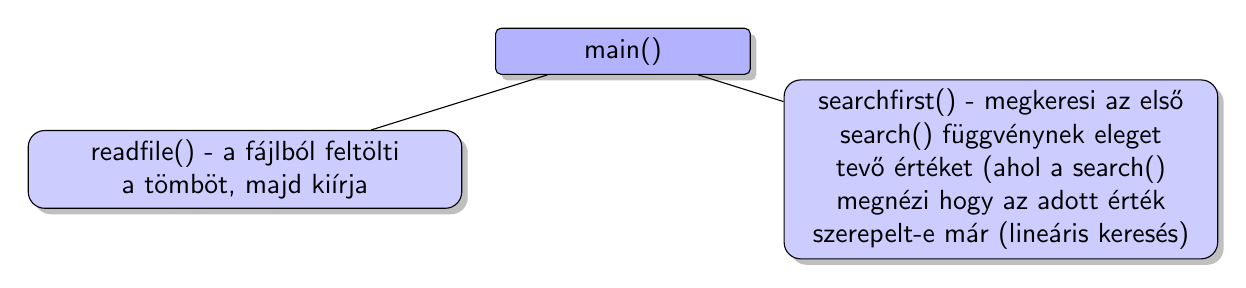
\begin{tikzpicture}[
  level 1/.style={sibling distance=96mm},
  edge from parent/.style={-,draw},
  >=latex]

% root of the the initial tree, level 1
\node[root] {main()}
% The first level, as children of the initial tree
  child {node[level 2] (c1) {readfile() - a fájlból feltölti a tömböt, majd kiírja}}
  child {node[level 2] (c7) {searchfirst() - megkeresi az első search() függvénynek eleget tevő értéket (ahol a search() megnézi hogy az adott érték szerepelt-e már (lineáris keresés)}};


\end{tikzpicture}
\paragraph{Tesztelési terv} \hspace{0pt} \\

\textit{\textbf{A feladat specifikációjára épülő (fekete doboz) tesztesetek:}}
\begin{itemize}[noitemsep]
\item \textbf{Lineáris keresés} tesztesetei:
\begin{itemize}[noitemsep]
\item \textbf{intervallum hossza} szerint
\begin{enumerate}[noitemsep]
\item \textit{nulla} hosszú: Egyetlen útlevélszám sincs. (üres vagy csak elválasztójelekből álló fájl - t3.txt: [] – Nincsen feltöltve a tömb, így nincs egy útlevélszám se.) 
\item \textit{egy} hosszú: Egyetlen útlevélszám van. (t6.txt - Legalább két elem kell a feltétel teljesüléséhez.)
\item \textit{kettő} hosszú: Két útlevélszám van. (t5.txt - a válasz PO118456 lesz)
\item \textit{több} hosszú: Több útlevélszám van. (t1.txt - a válasz AS123456 lesz)
\end{enumerate}
\end{itemize}
\begin{itemize}[noitemsep]
\item \textbf{intervallum eleje} szerint
\begin{enumerate}[noitemsep]
\item A keresett elem a legelső vizsgált elem. (t1.txt - a válasz AS123456 lesz)
\end{enumerate}
\end{itemize}
\begin{itemize}[noitemsep]
\item \textbf{intervallum vége} szerint
\begin{enumerate}[noitemsep]
\item A keresett elem a legutolsó vizsgált elem. (t2.txt - a válasz FF23423423 lesz)
\end{enumerate}
\end{itemize}
\begin{itemize}[noitemsep]
\item \textbf{tételre jellemző} esetek
\begin{enumerate}[noitemsep]
\item Egyetlen feltételnek eleget tevő szám sincs. (t9.txt)
\item Egyetlen feltételnek eleget tevő szám van. (t5.txt - a válasz PO118456 lesz)
\item Kettő feltételnek eleget tevő szám van. (t8.txt - a válasz AS123456 lesz.)
\item Több, a feltételnek eleget tevő szám van. (t10.txt)
\end{enumerate}
\end{itemize}
\item \textbf{Különleges értékek} esetei:
\begin{enumerate}[noitemsep]
\item Üres sorok, vagy túl kevés/túl sok karakterből álló stringek. (Ezt a beolvasás figyelmen kívül hagyja)
\end{enumerate}
\end{itemize}

\textit{\textbf{A megoldó programra épülő (fehér doboz) tesztesetek:}}
\begin{enumerate}[noitemsep]
  \item Hibás vagy nem létező állománynév megadása.
  \item Ismételt futtatás kipróbálása.
  \item Olyan állomány olvasása, ahol egy sorban több útlevélszám is található egyetlen illetve több szóközzel vagy tabulátor jellel elválasztva. (t4.txt)
  \item Olyan állomány olvasása, ahol minden szám külön sorban van. (t1.txt)
  \item Főprogram ciklusának ellenőrzése: olyan bemenő adatokkal, amelyekre a ciklus egyszer sem fut le (t3.txt), pontosan egyszer fut le (t5.txt), többször lefut és igazra értékelődik (t1.txt), többször lefut, de hamisre értékelődik (t7.txt).
\end{enumerate}
\end{document}